\documentclass[12pt,a4paper]{article}

\usepackage[utf8]{inputenc}
\usepackage[T1]{fontenc}

\usepackage[a4paper,margin=2.5cm]{geometry}
\usepackage{graphicx}
\usepackage{float}
\usepackage{booktabs}
\usepackage{hyperref}
\usepackage{xcolor}
\usepackage{amsmath}
\usepackage{caption}
\usepackage{titlesec}
\usepackage{parskip}
\usepackage{enumitem}

\hypersetup{
    colorlinks=true,
    linkcolor=black,
    urlcolor=blue,
    citecolor=black,
    pdftitle={Previsao de Resultados de Partidas Internacionais de Futebol},
    pdfauthor={Equipe do Projeto}
}

\titleformat{\section}{\large\bfseries}{\thesection}{1em}{}
\titleformat{\subsection}{\normalsize\bfseries}{\thesubsection}{1em}{}

\title{\textbf{Previsão de Resultados de Partidas Internacionais de Futebol \\
\large Um pipeline de Data Science aplicado ao dataset \\
\textit{International Football Results (1872--2026)}}}

\author{
  Murilo Kaemmerer Klein \\
  Guilherme Silveira Machado \\
  Samuel Vitor Zibetti \\
  \\
  \small Universidade de Passo Fundo (UPF) 
}

\date{}
\renewcommand{\contentsname}{Sumário}
\begin{document}

\begin{titlepage}
\centering

{\Large UPF -- Universidade de Passo Fundo\par}

\vspace{3cm}

{\LARGE\bfseries Previsão de Resultados de Partidas Internacionais de Futebol\par}

\vspace{0.8cm}

{\large Um pipeline de Data Science aplicado ao dataset\par}

\vspace{0.3cm}

{\itshape International Football Results (1872--2026)\par}

\vfill

{\large
Murilo Kaemmerer Klein\\
Guilherme Silveira Machado\\
Samuel Vitor Zibetti
\par}

\vfill

{\large
Passo Fundo -- RS\\
2026
\par}

\end{titlepage}

\section*{Resumo}

Este relatório descreve o desenvolvimento de um projeto completo de Data Science cujo objetivo é responder à pergunta: \emph{é possível prever o resultado de uma partida internacional de futebol (vitória do mandante, empate ou vitória do visitante) a partir do histórico de desempenho das seleções envolvidas?} Utilizando um dataset público com 49.425 partidas internacionais disputadas entre 1872 e 2026, construímos features de força das seleções (rating Elo calculado partida a partida), forma recente e histórico de confrontos diretos, e comparamos cinco algoritmos de classificação sob uma estratégia de validação temporal. O melhor modelo (\emph{Gradient Boosting}) atingiu 57,6\% de acurácia e F1-macro de 0,532, superando claramente um baseline ingênuo (47,3\% de acurácia, F1-macro de 0,214). Os resultados são consistentes com a literatura sobre previsão esportiva: o componente de aleatoriedade inerente ao futebol limita a acurácia atingível mesmo por modelos de mercado profissionais.

\clearpage

\tableofcontents

\clearpage


\section{Introdução}

O futebol é o esporte mais praticado e assistido do mundo, e a previsão de resultados de partidas é um problema de interesse tanto acadêmico (modelagem estatística de eventos esportivos) quanto prático (mercados de apostas, analítica esportiva, escalação de seleções). Diferentemente de esportes com placares mais altos, o futebol tem poucos gols por partida, o que torna o resultado mais sensível a fatores aleatórios (uma bola na trave, um pênalti duvidoso, uma lesão de última hora) e, consequentemente, mais difícil de prever de forma determinística.

O tema escolhido para este projeto é a \textbf{previsão de resultados de partidas internacionais de futebol} (vitória do mandante, empate ou vitória do visitante) a partir de características construídas sobre o histórico de desempenho das seleções: força relativa (rating Elo), forma recente e histórico de confrontos diretos entre as equipes.

\subsection{Relevância}

Diferente de ligas de clubes, partidas de seleções nacionais têm uma particularidade interessante para modelagem: o conjunto de "times" é fixo e relativamente pequeno (poucas centenas de seleções reconhecidas pela FIFA), os jogos são esparsos no tempo (em geral, poucas janelas internacionais por ano), e há uma forte dependência de competições oficiais (eliminatórias, Copas continentais, Copa do Mundo) que impõem estrutura adicional aos dados. Isso torna o problema tecnicamente interessante: o modelo precisa equilibrar sinal de longo prazo (força histórica da seleção) com sinal de curto prazo (forma recente), e lidar com classes desbalanceadas, já que empates são estatisticamente menos frequentes que vitórias.

\subsection{Questões e hipóteses iniciais}

O projeto foi guiado pelas seguintes questões, formuladas antes da análise
exploratória e testadas com os dados (Seção \ref{sec:eda}):

\begin{enumerate}[label=\textbf{H\arabic*.}]
    \item O número de partidas internacionais por ano cresceu substancialmente
    ao longo do tempo, refletindo a expansão e profissionalização do futebol
    internacional.
    \item Existe uma vantagem real de jogar em casa (mando de campo), que
    diminui quando a partida ocorre em campo neutro.
    \item Empates são a classe de resultado minoritária e, por isso, a mais
    difícil de prever.
    \item Um rating de força construído a partir do histórico de resultados
    (Elo) deve refletir o consenso atual sobre quais seleções são as mais
    fortes.
\end{enumerate}

\subsection{Repositório do projeto}

Todo o código-fonte, notebooks, dados e o dashboard interativo deste projeto estão disponíveis publicamente em:

\begin{center}
\url{https://github.com/muriloklein/trabalho_final_datascience}
\end{center}

% =====================================================================
\section{Dataset}
% =====================================================================

\subsection{Origem}

Os dados utilizados são provenientes do dataset público \href{https://www.kaggle.com/datasets/martj42/international-football-results-from-1872-to-2017}{\emph{International football results from 1872 to 2026}}, disponibilizado no Kaggle pelo usuário \texttt{martj42} e mantido a partir do repositório \href{https://github.com/martj42/international_results}{\texttt{martj42/international\_results}} no GitHub, sob licença \textbf{CC0 1.0} (domínio público). O dataset é atualizado continuamente; os dados utilizados neste trabalho foram coletados em junho de 2026 e cobrem partidas até 16/06/2026.

\subsection{Estrutura e dicionário de variáveis}

O arquivo principal (\texttt{results.csv}) contém uma linha por partida internacional masculina, com as seguintes variáveis originais:

\begin{center}
\small
\begin{tabular}{@{}ll@{}}
\toprule
\textbf{Variável} & \textbf{Descrição} \\
\midrule
\texttt{date} & Data da partida \\
\texttt{home\_team} & Seleção mandante \\
\texttt{away\_team} & Seleção visitante \\
\texttt{home\_score} & Gols marcados pela seleção mandante \\
\texttt{away\_score} & Gols marcados pela seleção visitante \\
\texttt{tournament} & Nome da competição (ex.: Copa do Mundo, amistoso) \\
\texttt{city}, \texttt{country} & Local da partida \\
\texttt{neutral} & Indica se a partida ocorreu em campo neutro \\
\bottomrule
\end{tabular}
\end{center}

Dois arquivos auxiliares também compõem o dataset: \texttt{shootouts.csv} (vencedores de disputas de pênaltis em partidas empatadas no tempo normal) e \texttt{former\_names.csv} (referência de mudanças de nome de seleções ao longo da história, como Alemanha Oriental/Ocidental $\rightarrow$ Alemanha).

Após a limpeza, o dataset contém \textbf{49.425 partidas} disputadas entre 30/11/1872 e 16/06/2026, envolvendo \textbf{336 seleções distintas}.

\subsection{Limpeza e transformações}

As seguintes etapas de limpeza e preparação foram aplicadas (implementadas em \texttt{src/data\_prep.py}):

\begin{enumerate}
    \item \textbf{Remoção de partidas sem placar:} o dataset inclui partidas futuras já agendadas (por exemplo, jogos da fase de grupos da Copa do Mundo de 2026, em andamento no momento da coleta) sem resultado ainda registrado. Essas linhas foram removidas do conjunto de treino/teste, pois não possuem rótulo (variável-alvo) disponível.
    \item \textbf{Conversão de tipos e ordenação cronológica:} datas convertidas para o tipo apropriado e o dataset ordenado por data, um pré-requisito indispensável para qualquer cálculo de feature baseada em histórico (ver Seção \ref{sec:features}).
    \item \textbf{Criação da variável-alvo (\texttt{outcome}):} categórica com três classes, derivada da diferença de gols (\texttt{home\_score} $-$ \texttt{away\_score}): \texttt{home\_win} (positiva), \texttt{draw} (zero) ou \texttt{away\_win} (negativa).
    \item \textbf{Categorização do tipo de torneio:} o campo \texttt{tournament} original possui centenas de valores distintos (cada copa regional, cada edição de torneio amistoso etc.). Esses valores foram agrupados em seis categorias relevantes para a modelagem: \emph{Friendly} (amistosos), \emph{WC Qualifiers} (eliminatórias da Copa do Mundo), \emph{Other Qualifiers} (outras eliminatórias), \emph{World Cup} (Copa do Mundo), \emph{Continental/Major} (Eurocopa, Copa América, Copa Africana de Nações etc.) e \emph{Regional/Minor Cup} (torneios regionais menores).
    \item \textbf{Recorte da amostra de modelagem:} optamos por restringir o conjunto de \emph{treino e teste} a partidas a partir do ano \textbf{2000} (25.363 partidas), evitando misturar a era moderna do futebol com períodos muito anteriores, em que o calendário de competições, o nível técnico e até as regras do jogo eram substancialmente diferentes. O histórico completo desde 1872, no entanto, é utilizado para \emph{inicializar} o cálculo de features de longo prazo, como o rating Elo e o histórico de confrontos diretos (Seção \ref{sec:features}).
\end{enumerate}

% =====================================================================
\section{Análise Exploratória}
\label{sec:eda}
% =====================================================================

A análise exploratória completa, com código e discussão célula a célula, está disponível em \texttt{notebooks/01\_EDA.ipynb}. Esta seção resume as principais descobertas, organizadas em torno das hipóteses formuladas na Introdução.

\subsection{H1: Crescimento do volume de partidas}

\begin{figure}[H]
    \centering
    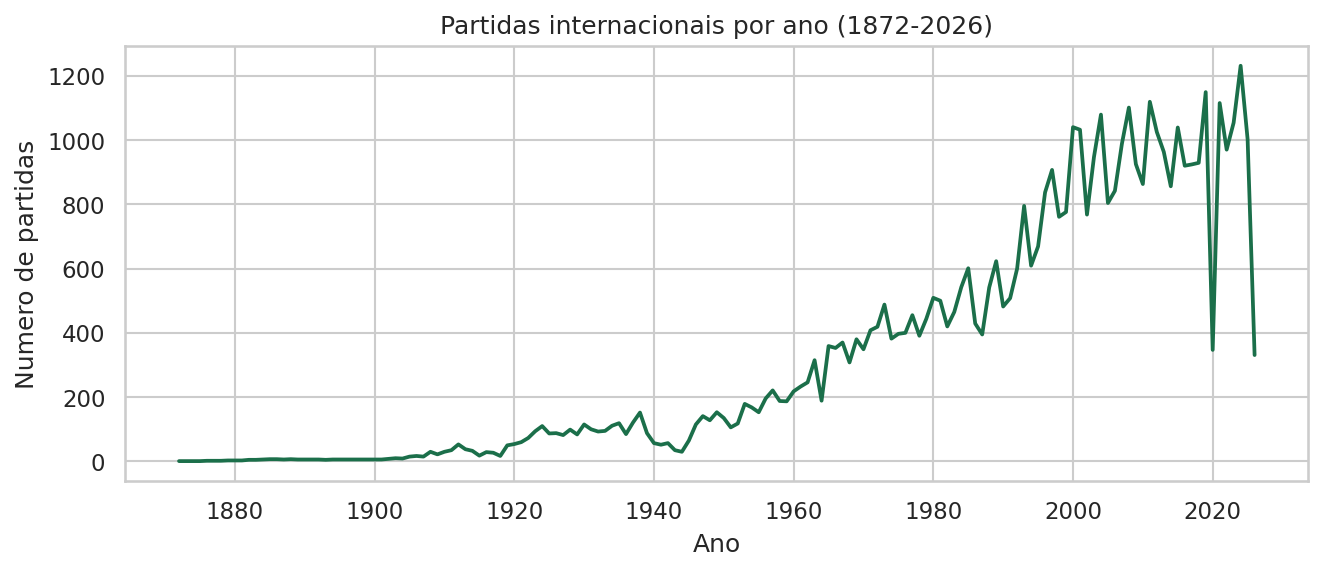
\includegraphics[width=0.85\textwidth]{01_matches_per_year.png}
    \caption{Número de partidas internacionais por ano (1872--2026).}
    \label{fig:matches_per_year}
\end{figure}

A Figura \ref{fig:matches_per_year} \textbf{confirma a hipótese H1}: o volume de partidas cresceu de poucas dezenas por ano no século XIX para mais de mil partidas anuais na era recente, refletindo a expansão da FIFA e a criação de competições regulares de eliminatórias. A queda visível em 2020 corresponde à pandemia de COVID-19, que cancelou ou postergou diversas janelas internacionais de jogos.

\subsection{H2: Vantagem de jogar em casa}

\begin{figure}[H]
    \centering
    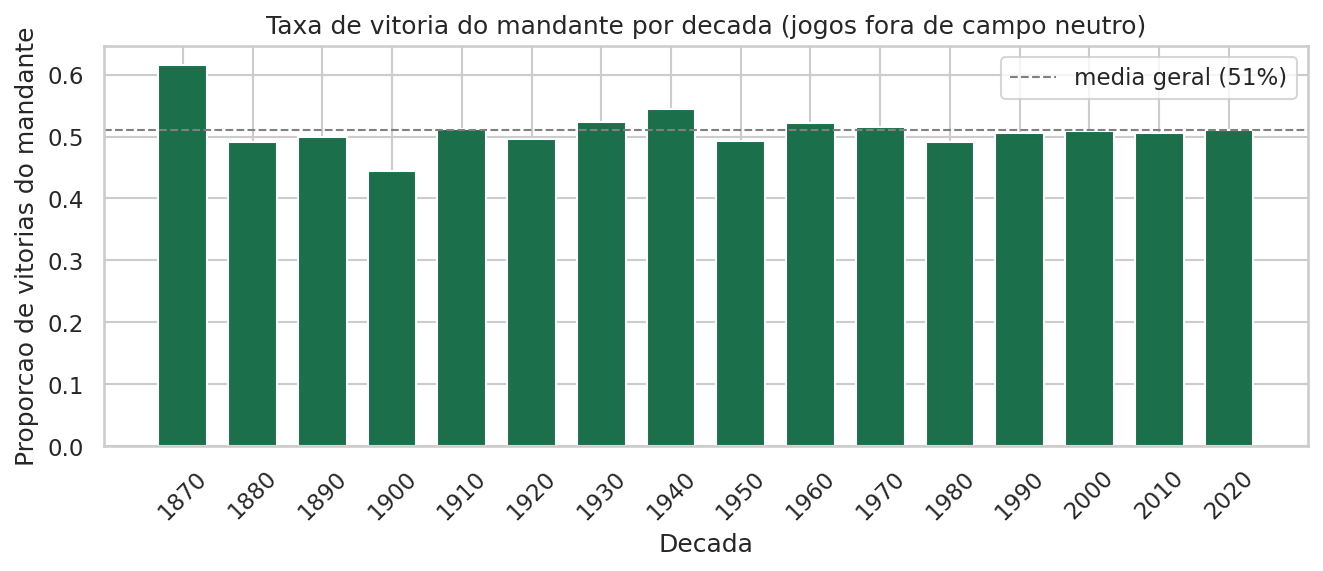
\includegraphics[width=0.85\textwidth]{03_home_advantage_by_decade.png}
    \caption{Taxa de vitória do mandante por década, considerando apenas
    partidas fora de campo neutro.}
    \label{fig:home_advantage}
\end{figure}

A taxa de vitória do mandante em partidas fora de campo neutro é de \textbf{50,7\%}, contra apenas \textbf{44,2\%} em partidas disputadas em campo neutro, uma diferença de mais de 6 pontos percentuais que \textbf{confirma a hipótese H2}. A vantagem de jogar em casa é real, persistente ao longo das décadas (Figura \ref{fig:home_advantage}) e justifica a inclusão tanto do mando de campo quanto da flag de campo neutro como features no modelo.

\subsection{H3: Desbalanceamento das classes}

\begin{figure}[H]
    \centering
    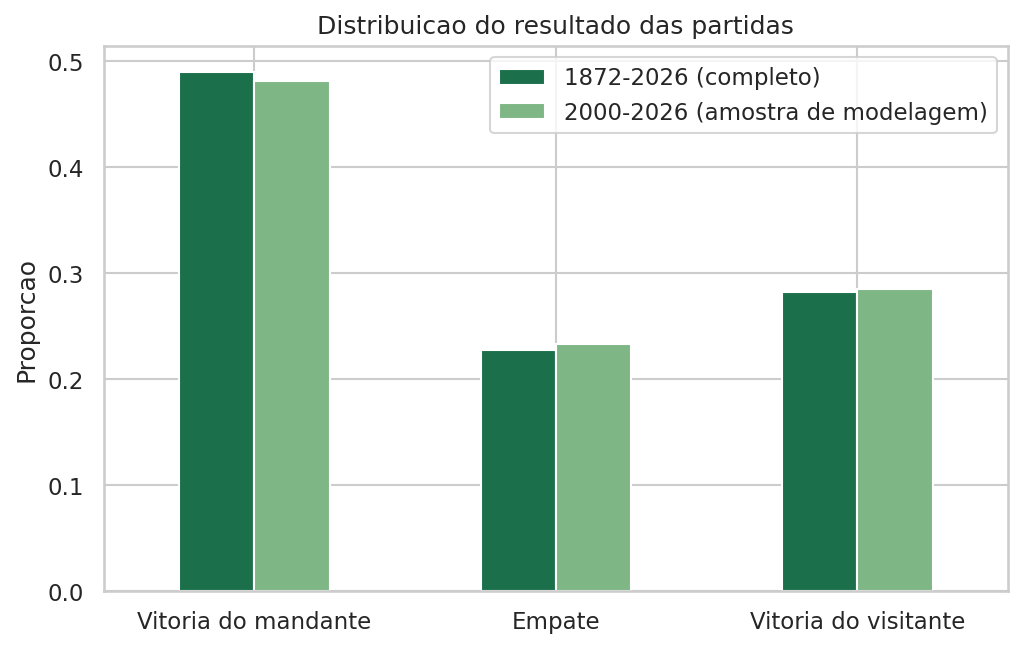
\includegraphics[width=0.7\textwidth]{02_outcome_distribution.png}
    \caption{Distribuição do resultado das partidas (amostra de modelagem,
    2000--2026, comparada ao histórico completo).}
    \label{fig:outcome_dist}
\end{figure}

Na amostra de modelagem (partidas a partir de 2000), os resultados se distribuem em \textbf{48,1\% de vitórias do mandante}, \textbf{28,5\% de vitórias do visitante} e apenas \textbf{23,3\% de empates} (Figura~\ref{fig:outcome_dist}), \textbf{confirmando a hipótese H3}. Esse desbalanceamento foi tratado na etapa de modelagem com a opção \texttt{class\_weight="balanced"} em todos os classificadores e com o uso da métrica F1-macro (que pondera igualmente todas as classes) em vez de apenas acurácia, evitando que o desempenho na classe minoritária seja mascarado.

\subsection{H4: Validação do rating Elo}

\begin{figure}[H]
    \centering
    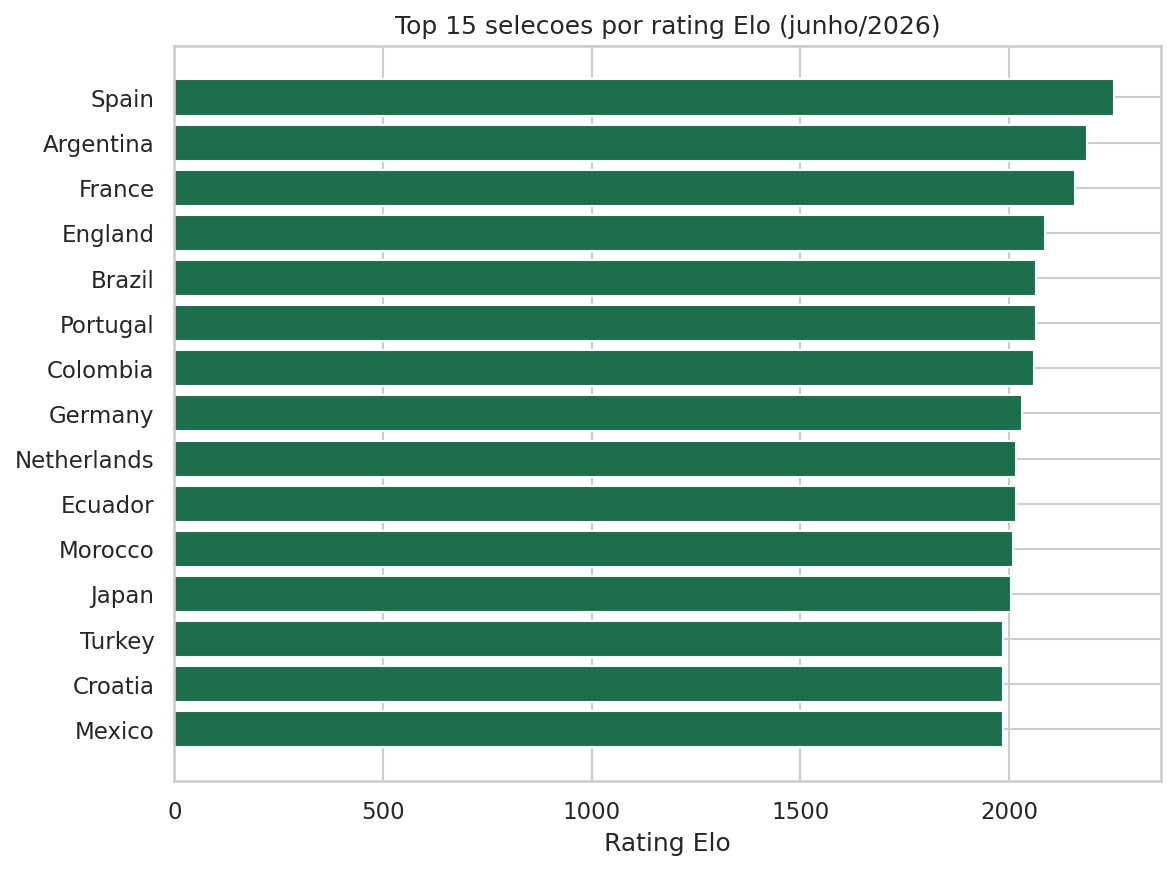
\includegraphics[width=0.7\textwidth]{04_top15_elo.png}
    \caption{Top 15 seleções por rating Elo calculado a partir dos dados
    (estado em junho de 2026).}
    \label{fig:top15_elo}
\end{figure}

O rating Elo construído a partir do histórico de resultados (metodologia detalhada na Seção \ref{sec:features}) posiciona Espanha, Argentina, França, Inglaterra e Brasil entre as cinco seleções mais fortes em junho de 2026 (Figura~\ref{fig:top15_elo}), um ranking consistente com o consenso público sobre as seleções mais competitivas do ciclo 2025--2026, \textbf{confirmando a hipótese H4}. Isso indica que o rating capturou sinal real de força das seleções, e não ruído, dando confiança para seu uso como feature no modelo preditivo.

% =====================================================================
\section{Modelagem}
% =====================================================================

\subsection{Engenharia de features}
\label{sec:features}

Para que o modelo aprenda a prever resultados a partir de informação genuinamente disponível \emph{antes} de cada partida, todas as features foram construídas com um cuidado metodológico central: \textbf{nenhuma feature pode usar informação que só existiria depois da partida em questão ter sido disputada} (vazamento temporal / \emph{data leakage}). As features implementadas (\texttt{src/features.py}) são:

\begin{itemize}
    \item \textbf{Rating Elo} (\texttt{elo\_diff}, \texttt{home\_elo\_pre}, \texttt{away\_elo\_pre}): calculado partida a partida, em ordem cronológica, desde 1872. O valor utilizado como feature é sempre o rating \emph{antes} da atualização correspondente àquela partida. O fator $K$ (taxa de ajuste do rating) varia conforme a importância do torneio (de 15 para amistosos a 45 para Copa do Mundo), e um pequeno bônus de mando de campo (60 pontos) é aplicado apenas para o cálculo da probabilidade esperada de vitória, seguindo a mesma lógica do \emph{World Football Elo Ratings}.
    \item \textbf{Forma recente} (taxa de vitórias e saldo de gols médio nas últimas 5 e 10 partidas de cada seleção): calculada com uma operação de \emph{shift} antes de qualquer agregação (\emph{rolling}), garantindo que a partida atual nunca seja incluída no próprio cálculo de sua feature.
    \item \textbf{Histórico de confrontos diretos} (\emph{head-to-head}): taxa histórica de vitórias do mandante especificamente contra aquele adversário, considerando apenas confrontos anteriores à data da partida.
    \item \textbf{Dias de descanso} desde o último jogo de cada seleção.
    \item \textbf{Categoria do torneio} e \textbf{campo neutro}, codificadas via \emph{one-hot encoding} e variável binária, respectivamente.
\end{itemize}

\subsection{Modelos e justificativa}

Foram comparados cinco modelos de classificação multiclasse (3 classes: \texttt{home\_win}, \texttt{draw}, \texttt{away\_win}):

\begin{center}
\small
\begin{tabular}{@{}ll@{}}
\toprule
\textbf{Modelo} & \textbf{Justificativa da escolha} \\
\midrule
Baseline (classe majoritária) & Referência mínima de comparação \\ Regressão Logística & Modelo linear interpretável, baseline robusto \\ Árvore de Decisão & Captura interações não-lineares simples, interpretável \\ Random Forest & \emph{Ensemble} robusto a overfitting \\ Gradient Boosting (\emph{HistGB}) & Geralmente o mais competitivo em dados tabulares \\
\bottomrule
\end{tabular}
\end{center}

Todos os modelos (exceto o baseline) foram treinados com \texttt{class\_weight="balanced"} para compensar o desbalanceamento das classes identificado na análise exploratória.

\subsection{Treinamento e validação}

A divisão entre treino e teste foi feita de forma \textbf{temporal, e não aleatória}: o conjunto de treino contém partidas até 2022 (21.745 partidas) e o conjunto de teste contém partidas de 2023 em diante (3.618 partidas). Essa escolha metodológica é central para a validade dos resultados: uma divisão aleatória (por exemplo, k-fold tradicional) misturaria partidas de diferentes épocas entre treino e teste, permitindo que o modelo "veja" indiretamente informação do futuro ao calcular features de forma recente e Elo para partidas do passado, além de não refletir o uso real do modelo, que é sempre prever jogos futuros a partir de dados estritamente anteriores.

% =====================================================================
\section{Resultados e Discussão}
% =====================================================================

\subsection{Comparação de modelos}

\begin{figure}[H]
    \centering
    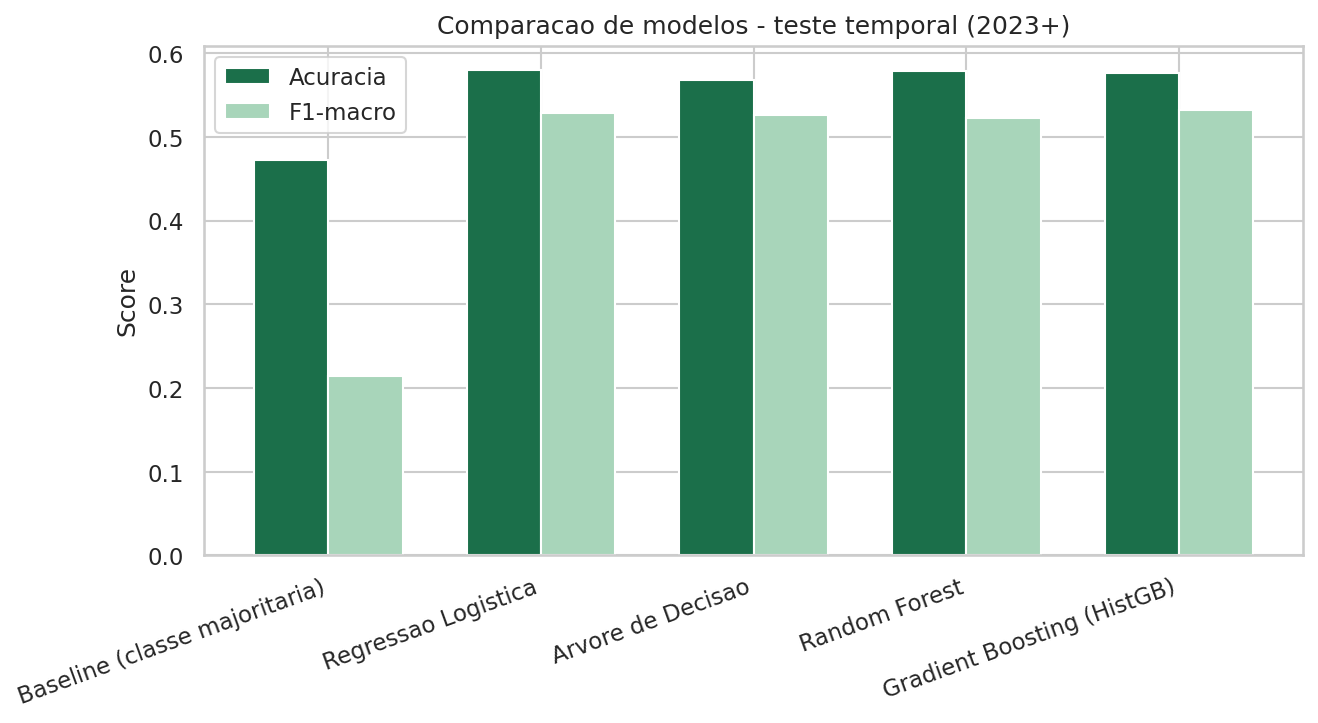
\includegraphics[width=0.85\textwidth]{05_model_comparison.png}
    \caption{Comparação de acurácia e F1-macro entre os modelos avaliados no
    conjunto de teste (partidas de 2023 em diante).}
    \label{fig:model_comparison}
\end{figure}

\begin{center}
\small
\begin{tabular}{@{}lcc@{}}
\toprule
\textbf{Modelo} & \textbf{Acurácia} & \textbf{F1-macro} \\
\midrule
Baseline (classe majoritária) & 47,3\% & 0,214 \\
Regressão Logística & 58,0\% & 0,528 \\
Árvore de Decisão & 56,8\% & 0,526 \\
Random Forest & 57,9\% & 0,523 \\
\textbf{Gradient Boosting (HistGB)} & \textbf{57,6\%} & \textbf{0,532} \\
\bottomrule
\end{tabular}
\end{center}

Todos os modelos superam claramente o baseline: a acurácia sobe de 47,3\% para a faixa de 57--58\%, e o F1-macro sobe de 0,214 para a faixa de 0,52--0,53. Um salto expressivo, já que o baseline ignora completamente as classes minoritárias (empate e vitória do visitante), prevendo sempre "vitória do mandante".

Entre os quatro modelos, a diferença de desempenho é pequena (no máximo cerca de 1 ponto percentual de acurácia entre eles). Esse padrão é esperado e consistente com a literatura sobre previsão de resultados esportivos: o resultado de uma partida de futebol tem um componente de aleatoriedade alto (lesões, decisões de arbitragem, um gol contra), e mesmo casas de apostas profissionais, que têm acesso a muito mais informação do que este projeto, incluindo escalações, lesões e o consenso do mercado de apostas, raramente ultrapassam 55--60\% de acurácia em previsões de resultado (vitória/empate/derrota). O \textbf{Gradient Boosting (HistGB)} foi selecionado como modelo final por apresentar o melhor F1-macro, sendo o modelo utilizado no dashboard interativo.

\subsection{Matriz de confusão e análise de erros}

\begin{figure}[H]
    \centering
    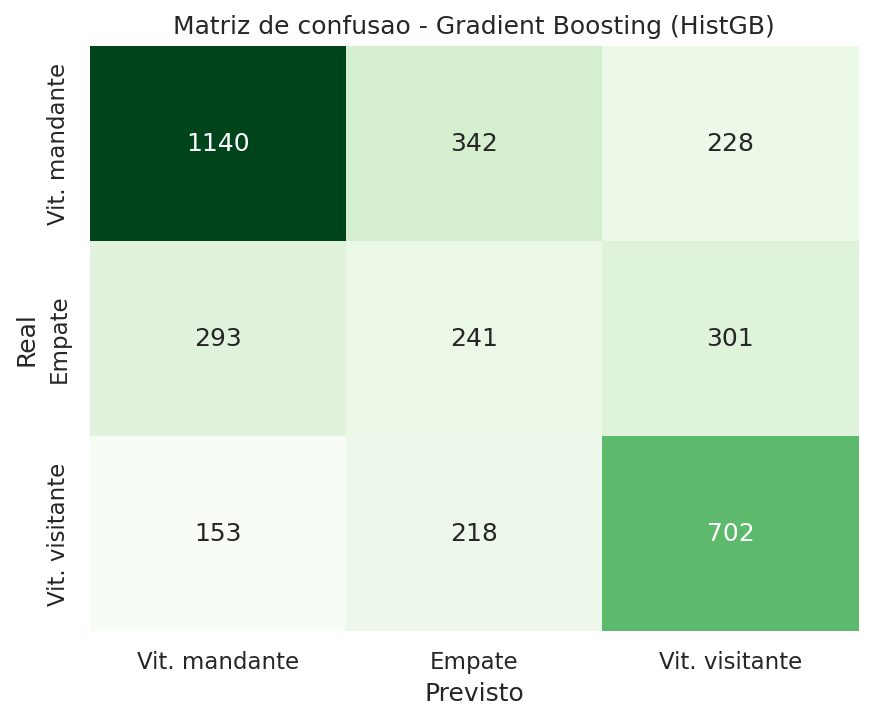
\includegraphics[width=0.55\textwidth]{06_confusion_matrix_best_model.png}
    \caption{Matriz de confusão do modelo final (Gradient Boosting) no
    conjunto de teste.}
    \label{fig:confusion_matrix}
\end{figure}

A matriz de confusão (Figura~\ref{fig:confusion_matrix}) confirma a hipótese H3 levantada na análise exploratória: \textbf{empates são, de fato, a classe mais difícil de prever}. O modelo atinge \emph{recall} de 66,7\% para vitórias do mandante e 65,4\% para vitórias do visitante, mas apenas \textbf{28,9\% de \emph{recall} para empates}, das 835 partidas que terminaram empatadas no conjunto de teste, o modelo só identificou corretamente 241. Isso é consistente com a natureza do problema: um empate frequentemente reflete um equilíbrio momentâneo e específico daquela partida (não necessariamente um padrão estrutural de longo prazo capturável a partir do histórico das equipes), tornando-o estatisticamente mais próximo de um evento "intermediário" entre as duas classes de vitória do que de uma categoria com identidade própria e bem definida nos dados.

\subsection{Importância das features}

A análise de importância de features (Random Forest, ver \texttt{notebooks/02\_modeling.ipynb}) mostra que a \textbf{diferença de rating Elo} entre as seleções (\texttt{elo\_diff}) é, isoladamente, a feature mais importante do modelo, seguida pelos ratings absolutos de cada seleção e pela taxa histórica de vitórias em confrontos diretos (\texttt{h2h\_home\_win\_rate}). Features de forma recente (últimos 5/10 jogos) têm peso menor que o rating Elo, sugerindo que a força estrutural de longo prazo de uma seleção é um preditor mais forte do que oscilações de curto prazo em seus resultados mais recentes, um resultado que valida o investimento feito na construção do rating Elo customizado, em vez de usar apenas identificadores categóricos de time.

% =====================================================================
\section{Dashboard Interativo}
% =====================================================================

Além do relatório escrito, foi desenvolvido um dashboard interativo em \textbf{Streamlit} (\texttt{dashboard/app.py}), organizado em três seções:

\begin{enumerate}
    \item \textbf{Explorar dados:} filtros por período, categoria de torneio e seleção, com gráficos de distribuição de resultados e evolução do
    rating Elo de seleções específicas ao longo do tempo.
    \item \textbf{Prever uma partida:} permite ao usuário escolher duas seleções (ou selecionar diretamente um confronto real ainda não disputado da Copa do Mundo de 2026, presente no próprio dataset) e visualizar a probabilidade prevista pelo modelo para cada resultado
    possível.
    \item \textbf{Desempenho dos modelos:} apresenta a tabela comparativa de métricas e a matriz de confusão do melhor modelo.
\end{enumerate}

Instruções para execução local do dashboard estão documentadas no
\texttt{README.md} do repositório.

% =====================================================================
\section{Conclusão}
% =====================================================================

Este projeto desenvolveu um pipeline completo de Data Science para prever resultados de partidas internacionais de futebol, cobrindo desde a coleta e limpeza de dados até a modelagem, avaliação e comunicação interativa dos resultados. As quatro hipóteses formuladas na etapa exploratória foram confirmadas pelos dados: o futebol internacional cresceu substancialmente em volume de partidas, existe uma vantagem real (e mensurável) de jogar em casa, empates são a classe de resultado minoritária e mais difícil de prever, e um rating de força construído inteiramente a partir do histórico de resultados reproduz o consenso atual sobre as seleções mais fortes do mundo.

O modelo final (Gradient Boosting) atingiu 57,6\% de acurácia e F1-macro de 0,532 em um conjunto de teste temporal rigoroso, superando substancialmente o baseline ingênuo. O ganho mais consistente, porém, não veio da escolha do algoritmo, a diferença entre os quatro modelos não-triviais foi pequena e sim da \textbf{engenharia de features}, em especial do rating Elo customizado, que se mostrou a variável mais informativa do modelo.

\subsection{Limitações}

O modelo desenvolvido não incorpora diversas informações que tipicamente melhoram a previsão de resultados esportivos: escalações e lesões de jogadores-chave, contexto tático (mudanças de técnico, esquema de jogo) e odds de mercado de apostas (que agregam informação privilegiada de milhares de apostadores). Além disso, a restrição da amostra de modelagem a partidas a partir do ano 2000, embora justificada metodologicamente, implica que o modelo não foi avaliado sobre a totalidade do histórico disponível.

\subsection{Trabalhos futuros}

Como extensões naturais deste trabalho, sugerimos: (i) incorporar dados de escalação e ausência de jogadores-chave, quando disponíveis; (ii) testar pesos de decaimento temporal nas features de forma recente, dando menos peso a jogos mais antigos dentro da própria janela; (iii) explorar um modelo de regressão para o placar exato (em vez de apenas o resultado), permitindo estimar probabilidades de múltiplos mercados (under/over, ambas marcam, etc.); e (iv) comparar o desempenho do modelo contra odds reais de casas de apostas, como benchmark externo de qualidade.

% =====================================================================
\appendix
\section*{Apêndice: Reprodutibilidade}
\addcontentsline{toc}{section}{Apêndice: Reprodutibilidade}
% =====================================================================

Todo o pipeline (limpeza, engenharia de features, treino e avaliação dos modelos) é executado por um único script (\texttt{run\_pipeline.py}) e foi validado de forma totalmente reprodutível a partir dos dados brutos. As instruções completas de instalação e execução, incluindo como rodar o dashboard localmente, estão documentadas no arquivo \texttt{README.md} do repositório do projeto.

\end{document}